\section{Durchführung}
\label{sec:Durchführung}
\subsection{Vorbereitung}
\label{subsec:Vorbereitung}
Um in der Auswertung die Ergebnisse mit den Literaturwerten vergleichen zu können,
soll zur Vorbereitung die Wärmeleitfähigkeit $\kappa$ für Aluminium, Messing und Edelstahl nachgeschlagen werden.
\begin{table}
    \centering
    \caption{Eigenschaften der Probestäbe.}
    \label{tab:}
    \begin{tabular}{c c c c c}
      \toprule
      {Material}  &  {Abmessung [cm] \cite{anleitung}}  &  {$\rho$ $[\si{\kilo\gram\per\meter\cubic}]$\cite{anleitung}}   &   {$c$ $[\si{\joule\per\kilo\gram\per\kelvin}]$\cite{anleitung}}  &   {$\kappa$ $[\si{\watt\per\meter\per\kelvin}]$\cite{chemie.de}}\\
      \midrule
      Messing (breit) & 9 x 1.2 x 0.4  & 8520   & 385 & 120\\
      Messing (schmal) & 9 x 0.7 x 0.4  & 8520  & 385 & 120\\
      Aluminium (breit) & 9 x 1.2 x 0.4 & 2800  & 830 & 237\\
      Edelstahl (breit) &  9 x 1.2 x 0.4  & 8000  & 400& 15 bis 21\\
      \bottomrule
    \end{tabular}
  \end{table}

\subsection{Versuchsaufbau}
\label{subsec:Versuchsaufbau}
\begin{figure}
    \centering
    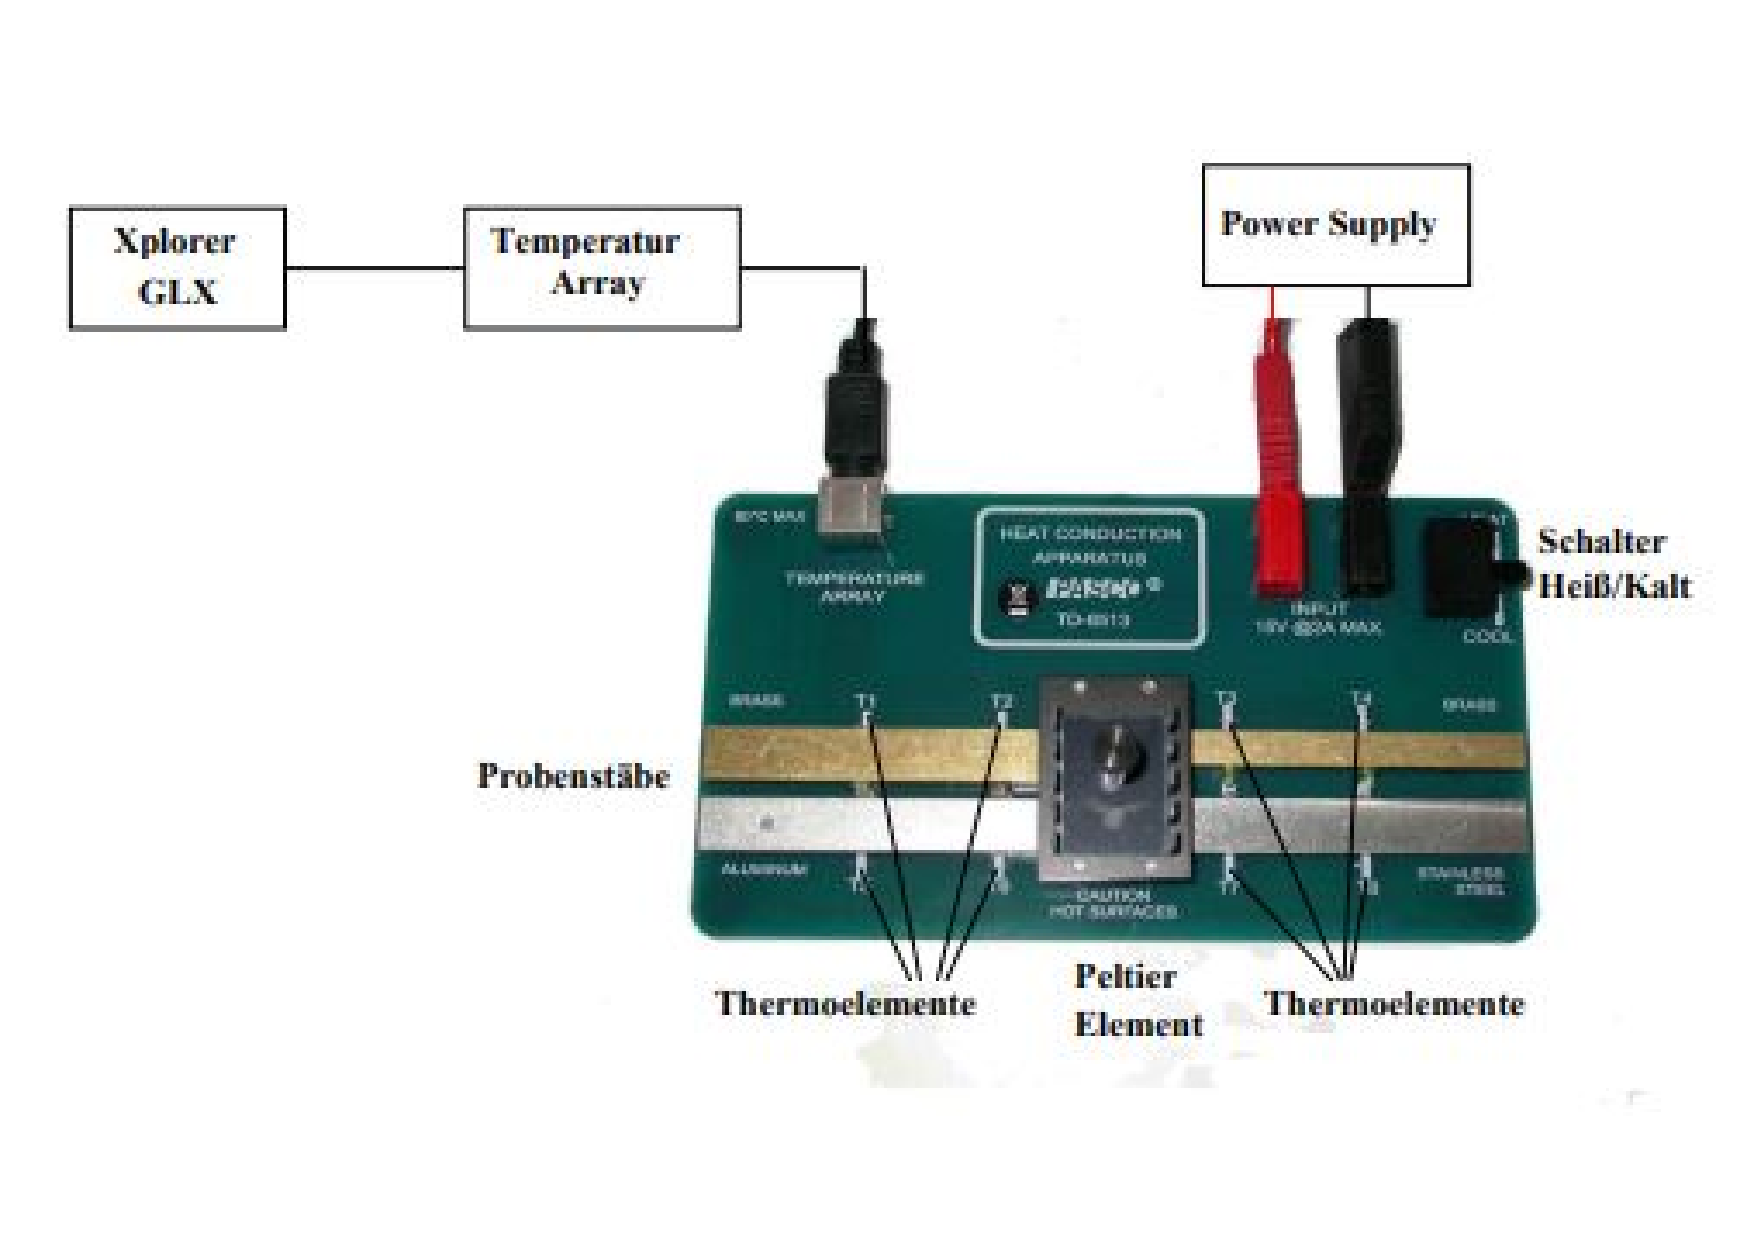
\includegraphics[width=\textwidth]{platine.pdf}
    \caption{Platine mit Probestäben.\cite{anleitung}}
    \label{fig:platine}
\end{figure}
Beide Methoden des Versuchs werden mit der Platine, die in Abbildung \ref{fig:platine} zu sehen ist, durchgeführt.
Auf der Platine sind die vier Probestäbe aus drei verschiedenen Materialien befestigt.
Aluminium, Edelstahl (stainless steel) und Messing (brass), wobei Messing zwei Mal in verschiedenen Größen zu finden ist.
Die Messstellen sind die Thermoelemente T1 bis T8.
T1 und T2 nimmt die Temperatur für Messing (breit) auf, T3 und T4 für Messing (schmal), T5 und T6 für Aluminium.
Die Temperatur für Edelstahl wird von T7 und T8 aufgenommen.
Der Abstand zwischen eines Thermoelementpaares beträgt $\SI{3}{\centi\metre}$.
Mit dem Schalter HEAT/COOL werden über das Peltierelement die Stäbe simultan geheizt bzw. gekühlt.
Über das Temperatur Array werden die Temperaturen an den Thermoelementen gespeichert.
Dafür wird das Xplorer GLX verwendet.
Für die statische Methode wird eine Spannung von $5\si{\volt}$ verwendet und für die dynamische Methode $8\si{\volt}$.

\subsection{Versuchsdurchführung}
\label{subsec:Versuchsdurchführung}
Vor jeder Messung wird am GLX die Abtastrate $\Delta t_\text{GLX}$ eingestellt und überprüft, ob alle acht Sensoren angezeigt werden.
Bei allen Messungen wird die Wärmeisolierung über die Probestäbe gelegt und alle acht Thermoelemente ausgelesen.
Sobald eine Messung beendet wird, wird der Schalter auf COOL gestellt und die Isolierung von den Stäben entfernt um diese zu kühlen.
Eine weitere Messung erfordert, dass alle Probestäbe auf unter $30\si{\celsius}$ abgekühlt sind.
\subsubsection{Statische Methode}
\label{subsubsec:statisch}
Die Abtastrate $\Delta t_\text{GLX}$ wird auf $5\si{\second}$ gestellt.
Die Eingangsspannung des Peltierelementes wird auf $5\si{\volt}$ eingestellt.
Die Messung wird gestartet und der Schalter auf HEAT gesetzt.
Wenn das Thermoelemente T7 eine Temperatur von ungefähr $45\si{\celsius}$ anzeigt,
wird die Messung beendet.
\subsubsection{Dynamische Methode}
\label{subsubsec:dynamisch}
Bei dem Angström-Messverfahren werden die Probestäbe periodisch geheizt und gekühlt.
Dazu wird zunächst die Abtastrate $\Delta t_\text{GLX}$ auf $2\si{\second}$ gestellt.
Die Eingangsspannung wird auf $8\si{\volt}$ eingestellt.

Im ersten Messdurchgang werden die Stäbe mit einer Periode von $80\si{\second}$ geheizt.
Somit wird mithilfe einer Stoppuhr der Schalter alle $40\si{\second}$ umgelegt, um zwischen Heizen und Kühlen zu wechseln.
Nach 12 Perioden wird die Messung beendet.

Im zweiten Messdurchgang soll die Periodendauer $200\si{\second}$ betragen.
Der Schalter wird alle $100\si{\second}$ umgelegt, hier wird auch eine Stoppuhr verwendet.
Die Messung wird beendet, sobald eines der Thermoelemente eine Temperatur von $80\si{\celsius}$ anzeigt.